% !TeX program = xelatex
\documentclass[a4paper,10pt]{article}

% ============================================================================
% កញ្ចប់បណ្ណាល័យ (Packages) – តាមលំនាំ NGS Preah Krasang Scenario (RAT23)
% ============================================================================
\usepackage[a4paper, left=0.95cm, right=0.95cm, top=0.85cm, bottom=0.92cm, footskip=0.50cm]{geometry}
\usepackage{amsmath, amssymb}
\usepackage{unicode-math}
\usepackage{fontspec}
\usepackage{array, longtable, multirow, colortbl}
\usepackage[table]{xcolor}
\usepackage{enumitem}
\usepackage{pifont}
\usepackage{fancyhdr}
\usepackage{tikz}
\usetikzlibrary{calc, arrows.meta, decorations.markings, positioning, babel}

% LaTeX 2025 + longtable v4.24 compatibility guard
\makeatletter
\let\@expl@@@mark@update@singlecol@structures@@\relax
\makeatother

% ============================================================================
% ការកំណត់ពុម្ពអក្សរ (Cross-Platform Windows + Cloud fonts/)
% ============================================================================
\providecommand{\NGSFindFonts}{%
  \IfFileExists{C:/Windows/Fonts/cambria.ttc}{%
    \def\NGSSysPath{C:/Windows/Fonts/}%
    \def\NGSUserPath{C:/Users/KIT/AppData/Local/Microsoft/Windows/Fonts/}%
  }{%
    \IfFileExists{./fonts/KhmerOSsiemreap.ttf}{\def\NGSSysPath{./fonts/}\def\NGSUserPath{./fonts/}}{%
    \IfFileExists{../fonts/KhmerOSsiemreap.ttf}{\def\NGSSysPath{../fonts/}\def\NGSUserPath{../fonts/}}{%
    \IfFileExists{../../fonts/KhmerOSsiemreap.ttf}{\def\NGSSysPath{../../fonts/}\def\NGSUserPath{../../fonts/}}{%
    \IfFileExists{../../../fonts/KhmerOSsiemreap.ttf}{\def\NGSSysPath{../../../fonts/}\def\NGSUserPath{../../../fonts/}}{%
    \IfFileExists{../../../../fonts/KhmerOSsiemreap.ttf}{\def\NGSSysPath{../../../../fonts/}\def\NGSUserPath{../../../../fonts/}}{%
    \IfFileExists{../../../../../fonts/KhmerOSsiemreap.ttf}{\def\NGSSysPath{../../../../../fonts/}\def\NGSUserPath{../../../../../fonts/}}{%
    \IfFileExists{../../../../../../fonts/KhmerOSsiemreap.ttf}{\def\NGSSysPath{../../../../../../fonts/}\def\NGSUserPath{../../../../../../fonts/}}{%
      \def\NGSSysPath{../../../../../../../fonts/}\def\NGSUserPath{../../../../../../../fonts/}%
    }}}}}}}%
  }%
}
\NGSFindFonts

\setmathfont[
  Path={\NGSSysPath},
  FontIndex=1,
  Scale=1.02
]{cambria.ttc}

\defaultfontfeatures{Ligatures=TeX}

\setmainfont[
  Path={\NGSUserPath},
  Extension=.ttf,
  Script=Khmer,
  BoldFont={KhmerOSsiemreap},
  BoldFeatures={FakeBold=1.8},
  ItalicFont={KhmerOSsiemreap},
  ItalicFeatures={FakeSlant=0.25},
  BoldItalicFont={KhmerOSsiemreap},
  BoldItalicFeatures={FakeBold=1.8, FakeSlant=0.25}
]{KhmerOSsiemreap}

\newfontfamily\muol[
  Path={\NGSUserPath},
  Extension=.ttf,
  Script=Khmer
]{KhmerOSmuollight}

\newfontfamily\TimesEn[
  Path={\NGSSysPath},
  Extension=.ttf,
  Scale=1.00,
  BoldFont={timesbd},
  ItalicFont={timesi},
  BoldItalicFont={timesbi}
]{times}

\newfontfamily\NagaBold[
  Path={\NGSUserPath},
  Extension=.ttf
]{AKbalthom Naga Bold}

\newfontfamily\CalibriFont[
  Path={\NGSSysPath},
  Extension=.ttf
]{calibri}

\newfontfamily\CourierBullet[
  Path={\NGSSysPath},
  Extension=.ttf
]{cour}
\newcommand{\wcirc}{{\CourierBullet\fontsize{9.2pt}{11pt}\selectfont o}}

\XeTeXlinebreaklocale "km"
\XeTeXlinebreakskip = 0pt plus 1pt minus 0.1pt

% ============================================================================
% ការកំណត់ពណ៌ និងទម្រង់ទំព័រ (Colors & Page Style)
% ============================================================================
\definecolor{stepgray}{HTML}{D9D9D9}
\definecolor{headgray}{HTML}{F2F2F2}
\definecolor{boxgray}{HTML}{D9D9D9}
\definecolor{darkred}{HTML}{C00000}
\definecolor{red5e}{HTML}{FF0000}

\pagestyle{fancy}
\fancyhf{}
\renewcommand{\headrulewidth}{0pt}
\fancyfoot[R]{\CalibriFont\fontsize{10.5pt}{12pt}\selectfont\thepage}

\setlength{\parindent}{0pt}
\setlength{\parskip}{0pt}
\setlength{\tabcolsep}{3.6pt}
\renewcommand{\arraystretch}{1.12}

\newcolumntype{L}[1]{>{\raggedright\arraybackslash}p{#1}}
\newcolumntype{C}[1]{>{\centering\arraybackslash}p{#1}}

% ============================================================================
% ម៉ាក្រូជំនួយ (Helper Macros)
% ============================================================================
\newcommand{\en}[1]{{\TimesEn #1}}
\newcommand{\enbf}[1]{{\TimesEn\textbf{#1}}}
\newcommand{\unit}[1]{\,\text{\en{#1}}}
\newcommand{\fiveE}[1]{{\NagaBold\fontsize{9.2pt}{12.5pt}\selectfont\textcolor{red5e}{#1}}}
\newcommand{\timenote}[1]{\textcolor{darkred}{\textit{#1}}}
\newcommand{\cnum}[1]{{\TimesEn\fontsize{10pt}{11.5pt}\selectfont\ding{\numexpr181+#1\relax}}\hspace{0.15em}}
\newcommand{\ditem}{\tikz[baseline=-0.5ex]\fill (0,0.40ex) -- (0.40ex,0) -- (0,-0.40ex) -- (-0.40ex,0) -- cycle;\hspace{0.25em}}
\newcommand{\cfig}[1]{\par\vspace{4pt}{\centering #1\par}\vspace{4pt}}

% រូបប្លង់ក្ដារខៀន ៣ ផ្នែក ស-ខ្មៅ សមាមាត្រច្បាស់ (~16.8 cm wide, font=\footnotesize)
\newcommand{\figBoardPlanRAT}{%
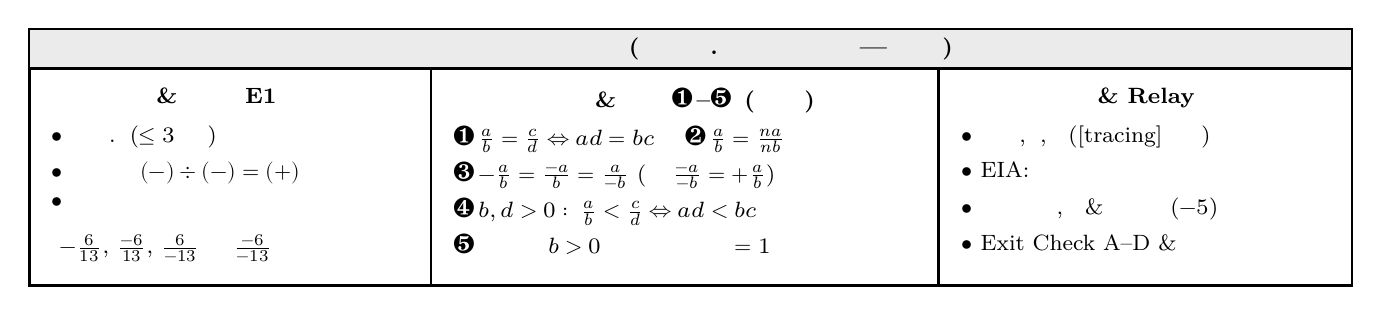
\begin{tikzpicture}[x=1cm, y=1cm, every node/.style={font=\footnotesize, text=black}]
  \draw[black, line width=1.05pt, fill=white] (0,-0.26) rectangle (16.80,3.00);
  \draw[black, line width=0.85pt] (5.10,-0.26) -- (5.10,2.50);
  \draw[black, line width=0.85pt] (11.55,-0.26) -- (11.55,2.50);
  \draw[black, line width=0.85pt, fill=gray!16] (0,2.50) rectangle (16.80,3.00);
  \node at (8.40,2.75) {\textbf{ប្លង់គ្រប់គ្រងក្ដារខៀន ៣ ផ្នែក (មេរៀនទី១៖ ២.៣ លក្ខណៈនៃចំនួនសនិទាន — ៥០ នាទី)}};

  % ផ្នែកឆ្វេង
  \node[anchor=north west] at (0.16,2.38) {\textbf{ផ្នែកទី១៖ រំលឹក \& បេសកកម្ម \en{E1}}};
  \node[anchor=north west] at (0.16,1.90) {$\bullet$ កំណែ ២.២ ($\le 3\text{ នាទី}$)};
  \node[anchor=north west] at (0.16,1.44) {$\bullet$ ក្បួនសញ្ញា $(-)\div(-)=(+)$};
  \node[anchor=north west] at (0.16,0.98) {$\bullet$ ស្លាកទឹកស្ពានកំពង់ស្វាយ៖};
  \node[anchor=north west] at (0.26,0.52) {$-\frac{6}{13},\,\frac{-6}{13},\,\frac{6}{-13}$ ធៀប $\frac{-6}{-13}$};

  % ផ្នែកកណ្ដាល
  \node[anchor=north west] at (5.26,2.38) {\textbf{ផ្នែកទី២៖ ខ្លឹមសារគោល \& ធនាគារ \cnum{1}--\cnum{5} (រក្សាទុក)}};
  \node[anchor=north west] at (5.26,1.90) {\cnum{1}$\frac{a}{b}=\frac{c}{d}\Leftrightarrow ad=bc$ \quad \cnum{2}$\frac{a}{b}=\frac{na}{nb}$};
  \node[anchor=north west] at (5.26,1.44) {\cnum{3}$-\frac{a}{b}=\frac{-a}{b}=\frac{a}{-b}$ (និង $\frac{-a}{-b}=+\frac{a}{b}$)};
  \node[anchor=north west] at (5.26,0.98) {\cnum{4}$b,d>0:\;\frac{a}{b}<\frac{c}{d}\Leftrightarrow ad<bc$};
  \node[anchor=north west] at (5.26,0.52) {\cnum{5}បង្រួមរួច៖ $b>0$ និង $\text{តួចែករួមធំបំផុត}=1$};

  % ផ្នែកស្ដាំ
  \node[anchor=north west] at (11.72,2.38) {\textbf{ផ្នែកទី៣៖ លំហាត់គំរូ \& \en{Relay}}};
  \node[anchor=north west] at (11.72,1.90) {$\bullet$ គំរូ ក, ខ, គ (\en{[tracing]} ខ្វែង)};
  \node[anchor=north west] at (11.72,1.44) {$\bullet$ \en{EIA}: គុណខ្វែង ធៀប សម្រួលមុន};
  \node[anchor=north west] at (11.72,0.98) {$\bullet$ ប្រតិបត្តិ ក, ខ \& លំហាត់ ១ ($-5$)};
  \node[anchor=north west] at (11.72,0.52) {$\bullet$ \en{Exit Check A--D} \& កិច្ចការផ្ទះ};
\end{tikzpicture}}

\begin{document}
\fontsize{9.8pt}{14.6pt}\selectfont

% ============================================================================
% ក្បាលទំព័រ (Header & Metadata)
% ============================================================================
\begin{center}
{\muol\fontsize{11pt}{15pt}\selectfont សេណារីយ៉ូនៃការបង្រៀន \enbf{(Teaching Scenario -- RAT23)}}
\end{center}
\vspace{2pt}

\noindent\begin{tabular}{|L{2.00cm}|L{6.75cm}|L{1.85cm}|L{7.40cm}|}
\hline
\rowcolor{headgray}
\textbf{សាលារៀន៖} & អនុវិទ្យាល័យព្រះក្រសាំង (កំពង់ស្វាយ--កំពង់ធំ) & \textbf{មុខវិជ្ជា៖} & គណិតវិទ្យា ថ្នាក់ទី៨ (ផ្នែកពីជគណិត) \\
\hline
\textbf{មេរៀន៖} & \textbf{មេរៀនទី១៖ ចំនួនសនិទាន — ២.៣. លក្ខណៈ} & \textbf{រយៈពេល៖} & \textcolor{darkred}{\textbf{១ ម៉ោងសិក្សា (៥០ នាទី)}} \en{|} ទំព័រ ៥ និង ១១ \\
\hline
\textbf{គ្រូបង្រៀន៖} & ហុក ប៊ុនថែន & \textbf{កាលបរិច្ឆេទ៖} & ថ្ងៃចន្ទ ទី១៦ ខែវិច្ឆិកា ឆ្នាំ២០២៦ (៧កើត ខែកត្តិក ២៥៧០) \\
\hline
\end{tabular}

\vspace{4pt}
{\muol ផ្នែកទី ១៖ លំដាប់ឈុតឆាកបង្រៀន ៥០ នាទី \enbf{(}បែងចែកតាមនាទី\enbf{-}ទល់\enbf{-}នាទី\enbf{)}}
\vspace{2pt}

% ============================================================================
% ផ្នែកទី ១៖ តារាងឈុតឆាក (Granular Sub-Rows for >=90% Page Fill)
% ============================================================================
\begin{longtable}{|C{1.30cm}|L{2.70cm}|C{0.90cm}|L{8.15cm}|L{4.55cm}|}
\hline
\rowcolor{stepgray}
\textbf{ម៉ោង} & \textbf{ឈុត / ជំហាន \enbf{5E}} & \textbf{នាទី} & \textbf{សកម្មភាពបង្រៀន និងសំណួរ--ចម្លើយគំរូ (គ្រូ--សិស្ស)} & \textbf{សម្ភារៈ និងកំណត់ចំណាំ / \enbf{Warrant}} \\
\hline
\endfirsthead
\hline
\rowcolor{stepgray}
\textbf{ម៉ោង} & \textbf{ឈុត / ជំហាន \enbf{5E}} & \textbf{នាទី} & \textbf{សកម្មភាពបង្រៀន និងសំណួរ--ចម្លើយគំរូ (គ្រូ--សិស្ស)} & \textbf{សម្ភារៈ និងកំណត់ចំណាំ / \enbf{Warrant}} \\
\hline
\endhead
\hline
\endfoot
\hline
\endlastfoot

% --- ឈុតទី១ (00-02) ---
\en{00--02} &
\textbf{ឈុតទី ១}\par
ជំហានទី១៖ រដ្ឋបាលថ្នាក់ &
២ &
\ditem គ្រូពិនិត្យអវត្តមាន អនាម័យ និងរៀបចំសិស្សជាក្រុម ៤ នាក់ («ក្រុមអ្នកស៊ើបអង្កេតចំនួនសនិទាន»)។\par\vspace{2pt}
\ditem \textbf{គ្រូ៖} «សូមដាក់សន្លឹកពិសោធន៍ \en{P1} ផ្កាប់មុខលើតុ និងត្រៀមបន្ទាត់ \en{cm} ខ្មៅដៃ!» &
\wcirc\ ចែកសន្លឹក \en{P1 (1:1)} និងបិទផ្ទាំងធនាគារ \cnum{1}--\cnum{5} (\en{P4}) លើក្ដារខៀន។ \\[3pt]
\hline

% --- ឈុតទី២ (02-08) ---
\en{02--05} &
\textbf{ឈុតទី ២ក}\par
ជំហានទី២៖ កំណែកិច្ចការផ្ទះ &
៣ &
\ditem គ្រូហៅសិស្សផ្ទៀងផ្ទាត់ចម្លើយសង្ខេបនៃកិច្ចការផ្ទះមេរៀន ២.២៖\par\vspace{2pt}
\hspace*{0.3em}១) $-\frac{3}{2} < -0.5 < -\frac{1}{4} < 0.75 < \frac{5}{4} < 1\frac{1}{2}$\par\vspace{2pt}
\hspace*{0.3em}២) $0.\overline{4}=\frac{4}{9} < 0.8\overline{21}=\frac{271}{330} < 1.\overline{285}=\frac{428}{333}$ \; ; \; ៣) $\frac{9}{20}, \frac{11}{20}$។ &
\wcirc\ គ្រប់គ្រងពេល $\le 3$ នាទី។\par\vspace{2pt}
\wcirc\ គូសបន្ទាត់ចំនួនផ្ទៀងរហ័សនៅផ្នែកទី១ ក្ដារខៀន។ \\[3pt]

\en{05--08} &
\textbf{ឈុតទី ២ខ}\par
ជំហានទី២៖ រំលឹកមូលដ្ឋាន &
៣ &
\ditem \textbf{គ្រូ៖} «តើ $(-6)\times(-13)$ និង $(-25)\div(-5)$ មានសញ្ញាអ្វី? ចុះ $\text{តួចែករួមធំបំផុត }(15,36)$ ស្មើប៉ុន្មាន?»\par\vspace{2pt}
\ditem \textbf{សិស្ស៖} «សញ្ញាបូកទាំងពីរ ($+78$ និង $+5$) ហើយតួចែករួមធំបំផុតគឺ $3$!» &
\wcirc\ រំលឹកក្បួន $(-)\div(-)=(+)$ បង្ការកំហុសក្នុង \en{POE 2A} និងគំរូ (ខ)។ \\[3pt]
\hline

% --- ឈុតទី៣ (08-11: E1) ---
\en{08--11} &
\textbf{ឈុតទី ៣}\par
\fiveE{E1 - Engage}\par
បេសកកម្មស្ពានកំពង់ស្វាយ &
៣ &
\ditem គ្រូបង្ហាញបង្គោលវាស់ទឹកទិសឈរក្រោមស្ពានកំពង់ស្វាយ និងអ័ក្សផ្អៀង $140^\circ$ ដែលមានស្លាក ៤៖ $-\frac{6}{13}\unit{m},\; \frac{-6}{13}\unit{m},\; \frac{6}{-13}\unit{m},\; \frac{-6}{-13}\unit{m}$។\par\vspace{2pt}
\ditem \textbf{គ្រូ៖} «តើស្លាកណាខ្លះស្ថិតនៅជម្រៅដូចគ្នាបេះបិទក្រោម $0\unit{m}$ ហើយស្លាកណាមួយលោតទៅលើ $0\unit{m}$?»\par\vspace{2pt}
\ditem \textbf{សិស្ស៖} ទស្សន៍ទាយខុសៗគ្នា។ គ្រូកត់សំឡេងឆ្នោតលើក្ដារខៀន \textbf{ដោយមិនទាន់ប្រាប់ចម្លើយ}។ &
\wcirc\ បរិបទពិតក្នុងស្រុកកំពង់ស្វាយ (\en{Barrera-Mora \& Reyes-Rodriguez, 2019})។\par\vspace{2pt}
\wcirc\ រក្សាចម្លើយទុកផ្ទៀងនៅ \fiveE{E5}។ \\[3pt]
\hline

% --- ឈុតទី៤ (11-22: E2) ---
\en{11--15} &
\textbf{ឈុតទី ៤ក}\par
\fiveE{E2 - Explore}\par
បន្ទះសមមូល \en{1:1} &
៤ &
\ditem គ្រូឱ្យសិស្សផ្ងារសន្លឹក \en{P1 (Actual Size 100\%)} វាស់បន្ទះផ្ទៀង $5.00\unit{cm}$ រួចផ្ទឹមបន្ទះ $\frac{5}{7}$ ($5.00\unit{cm}$ នៃ $7.00\unit{cm}$) ជាមួយបន្ទះក្រឡា $\frac{25}{35}$ ($25\times 2\unit{mm}=5.00\unit{cm}$)។\par\vspace{2pt}
\ditem \textbf{សិស្ស៖} ឃើញប្រវែងស្មើគ្នា ហើយគណនា $\frac{-25}{-35}=\frac{(-5)\times 5}{(-5)\times 7}=\frac{5}{7}$ និង $(-25)\times 7 = (-35)\times 5 = -175$។ &
\wcirc\ ផ្សារភ្ជាប់រូបភាពផ្នែក-ទាំងមូល ទៅនិមិត្តសញ្ញា (\en{Tucker, 2014; Ertuna \& Toluk Uçar, 2021})។ \\[3pt]

\en{15--18} &
\textbf{ឈុតទី ៤ខ}\par
\fiveE{E2 - Explore}\par
\en{POE 2A} (ឆ្លុះសញ្ញា) &
៣ &
\ditem \textbf{ទស្សន៍ទាយ (\en{P})៖} «តើ $-\frac{2}{3}$ ស្មើនឹង $\frac{-2}{-3}$ ដែរឬទេ?»\par\vspace{2pt}
\ditem \textbf{សង្កេត និងពន្យល់ (\en{O--E})៖} សិស្សបត់បន្ទាត់ចំនួន \en{1:1} ($1\text{ ឯកតា}=6.00\unit{cm}$) ត្រង់គល់ $0$៖ ឃើញ $-\frac{2}{3}=\frac{-2}{3}=\frac{2}{-3}$ នៅ $-4.00\unit{cm}$ (ឆ្វេង $0$) ឯ $\frac{-2}{-3}=+\frac{2}{3}$ ឆ្លុះទៅ $+4.00\unit{cm}$ (ស្ដាំ $0$)! &
\wcirc\ បំបែកការយល់ច្រឡំចែកសញ្ញាដកទៅទាំងលើទាំងក្រោម (\en{Yetim \& Alkan, 2013; Lee \& Boyadzhiev, 2020})។ \\[3pt]

\en{18--22} &
\textbf{ឈុតទី ៤គ}\par
\fiveE{E2 - Explore}\par
\en{POE 2B} (អន្ទាក់ $b<0$) &
៤ &
\ditem \textbf{ទស្សន៍ទាយ (\en{P})៖} «ប្រៀបធៀប $\frac{1}{-2}$ និង $\frac{1}{3}$៖ បើគុណខ្វែងភ្លាម $1\times 3=3 > (-2)\times 1=-2$ តើ $\frac{1}{-2}>\frac{1}{3}$ មែនទេ?»\par\vspace{2pt}
\ditem \textbf{សង្កេត និងពន្យល់ (\en{O--E})៖} លើបន្ទាត់ចំនួន \en{1:1} ចំណុច $\frac{1}{-2}=-3.00\unit{cm}$ នៅឆ្វេង $\frac{1}{3}=+2.00\unit{cm}$ ដូច្នេះ $\frac{1}{-2}<\frac{1}{3}$! សិស្សរកឃើញថា មុនគុណខ្វែងវិសមភាព ត្រូវប្ដូរឱ្យ $b>0, d>0$ ជាមុន ($\frac{-1}{2}<\frac{1}{3}\Leftrightarrow -3<2$)។ &
\wcirc\ \textbf{ចំណុចគន្លឹះ \en{Pause-Ask}៖} ទប់ស្កាត់កំហុសគុណខ្វែងដោយភ្លេចសញ្ញាភាគបែង (\en{Çetin, 2022}: $25\%$ ខុស)។ \\[3pt]
\hline

% --- ឈុតទី៥ (22-28: E3) ---
\en{22--28} &
\textbf{ឈុតទី ៥}\par
\fiveE{E3 - Explain}\par
សំយោគលក្ខណៈ \cnum{1}--\cnum{5} &
៦ &
\ditem តំណាងក្រុមឡើងបង្គុំលក្ខណៈទាំង ៤ (សៀវភៅទំព័រ ៥) ភ្ជាប់ផ្ទាំងធនាគារហេតុផល \cnum{1}--\cnum{5} (\en{P4})៖\par\vspace{2pt}
\hspace*{0.3em}\cnum{1}$\frac{a}{b}=\frac{c}{d}\Leftrightarrow ad=bc$ \quad \cnum{2}$\frac{a}{b}=\frac{na}{nb}\;(n\neq 0)$ \quad \cnum{3}$-\frac{a}{b}=\frac{-a}{b}=\frac{a}{-b}$\par\vspace{2pt}
\hspace*{0.3em}\cnum{4}$b>0,d>0:\;\frac{a}{b}<\frac{c}{d}\Leftrightarrow ad<bc$ \quad \cnum{5}បង្រួមរួច៖ $b>0$ និង $\text{តួចែករួមធំបំផុត }(|a|,b)=1$។\par\vspace{2pt}
\ditem គ្រូសង្ខេបតារាង «សម្មតិកម្ម--សន្និដ្ឋាន--វិបាក» នៅផ្នែកកណ្ដាលក្ដារខៀន។ &
\wcirc\ រៀបចំជារចនាសម្ព័ន្ធ \en{Hub-and-Spoke} (\en{Xu et al., 2026}) កាត់បន្ថយការទន្ទេញដាច់ៗពីគ្នា។ \\[3pt]
\hline

% --- ឈុតទី៦ (28-38: E4) ---
\en{28--33} &
\textbf{ឈុតទី ៦ក}\par
\fiveE{E4 - Elaborate}\par
លំហាត់គំរូ ក, ខ &
៥ &
\ditem ចែកកាតស៊ើបអង្កេត ៣ ជំហាន \en{P2}។ គ្រូដឹកនាំគំរូត្រឹមត្រូវ (\en{CE}) លើ \textbf{ក.} $\frac{6}{-13}, \frac{-6}{13}$៖ ១) ព័ទ្ធរង្វង់សញ្ញាដក \cnum{3}; ២) ចង្អុលអូសខ្វែង \en{[tracing]} $6\times 13 = (-13)\times(-6) = 78$ \cnum{1}; ៣) ជ្រើសទម្រង់បង្រួមរួច $\frac{-6}{13}$ \cnum{5} (ព្រោះ $b=13>0$)។\par\vspace{2pt}
\ditem សិស្សធ្វើ \textbf{ខ.} $\frac{-25}{-35}, \frac{5}{7}$ ជាគូ៖ សម្រួលនឹង $-5$ តាម \cnum{2} បានទម្រង់បង្រួមរួច $\frac{5}{7}$។ &
\wcirc\ បង្ហាញគំរូត្រឹមត្រូវ (\en{CE}) មុនអន្ទាក់កំហុស (\en{Wesenberg et al., 2022}) + \en{[tracing]} (\en{Yeo \& Tzeng, 2019})។ \\[3pt]

\en{33--38} &
\textbf{ឈុតទី ៦ខ}\par
\fiveE{E4 - Elaborate}\par
លំហាត់គំរូ គ \& \en{EIA} &
៥ &
\ditem សិស្សដោះស្រាយ \textbf{គ.} $\frac{-15}{36}, \frac{20}{-48}$៖ អូសខ្វែង $(-15)\times(-48)=36\times 20=720$ \cnum{1} រួចសម្រួល $\div 3$ បានទម្រង់បង្រួមរួច $\frac{-5}{12}$ \cnum{5}។\par\vspace{2pt}
\ditem \textbf{សំណួរ \en{EIA Looking-Back}៖} «បើយើងសម្រួល $\frac{-15}{36}=\frac{-5}{12}$ និង $\frac{20}{-48}=\frac{-5}{12}$ មុន តើចំណេញអ្វីខ្លះធៀបនឹងការគុណ $36\times 20=720$?» សិស្ស៖ «លេខតូច ងាយគិត បានចម្លើយទាំងពីរក្នុងពេលតែមួយ!» &
\wcirc\ ពង្រឹងការពន្យល់ខ្លួនឯង (\en{Barbieri et al., 2022}) និងជម្រើសយុទ្ធសាស្ត្របត់បែន។ \\[3pt]
\hline

% --- ឈុតទី៧ (38-48: E5) ---
\en{38--44} &
\textbf{ឈុតទី ៧ក}\par
\fiveE{E5 - Evaluate}\par
\en{Relay} ប្រតិបត្តិ \& លំហាត់ ១ &
៦ &
\ditem ចែកសន្លឹក \en{Relay P3}៖ សមាជិកទី១ រៀបសញ្ញា \cnum{3}, ទី២ ផ្ទៀងសមមូល \cnum{1}/\cnum{2}, ទី៣ សរសេរទម្រង់បង្រួមរួច \cnum{5}, ទី៤ ត្រួតពិនិត្យពេលគ្រូហៅ \textbf{\en{Pause-Review}}៖\par\vspace{2pt}
\hspace*{0.3em}-- \textbf{ប្រតិបត្តិ (ទំ.៥)៖} ក. $\frac{16}{-30}=\frac{-8}{15}$ ($240=240$, បង្រួមរួច $\frac{-8}{15}$); ខ. $\frac{-15}{-35}=\frac{21}{49}$ (បង្រួមរួច $\frac{3}{7}$)។\par\vspace{2pt}
\hspace*{0.3em}-- \textbf{លំហាត់ ១ (ទំ.១១)៖} ចំនួនស្មើ $-5$ គឺ $\frac{-5}{1},\; \frac{5}{-1},\; -\frac{5}{1},\; -\frac{-5}{-1}$ (សញ្ញាដកសេស)។ &
\wcirc\ ផ្ទៀងបិទបេសកកម្ម \fiveE{E1} ស្ពានកំពង់ស្វាយ៖ $\frac{-6}{-13}=+\frac{6}{13}$ ខុសពីស្លាក ៣ ទៀត! \\[3pt]

\en{44--48} &
\textbf{ឈុតទី ៧ខ}\par
\fiveE{E5 - Evaluate}\par
\en{Exit Check A--D} &
៤ &
\ditem សិស្សលើកបណ្ណ \en{A--D (P5)} ព្រមគ្នាក្នុងរយៈពេល ៩០ វិនាទី៖\par\vspace{2pt}
\hspace*{0.3em}-- សំណួរទី១៖ ទម្រង់បង្រួមរួចនៃ $\frac{18}{-42}$ $\rightarrow$ ចម្លើយត្រូវ \textbf{\en{C}} ($\frac{-3}{7}$); អន្ទាក់ \en{A} ទុក $b<0$, \en{B} ដកពីរជាន់, \en{D} សម្រួលមិនអស់។\par\vspace{2pt}
\hspace*{0.3em}-- សំណួរទី២៖ ជំហានទី១ ប្រៀបធៀប $\frac{3}{-4}$ និង $\frac{-5}{7}$ $\rightarrow$ ចម្លើយត្រូវ \textbf{\en{B}} (ប្ដូរ $\frac{3}{-4}=\frac{-3}{4}$ មុនគុណខ្វែង)។ &
\wcirc\ កត់ត្រាចំនួនបណ្ណខុសភ្លាមៗ ដើម្បីកែតម្រូវមុនចេញពីថ្នាក់ (\en{Van et al., 2018})។ \\[3pt]
\hline

% --- ឈុតទី៨ (48-50: Step 5) ---
\en{48--50} &
\textbf{ឈុតទី ៨}\par
ជំហានទី៥៖ កិច្ចការផ្ទះ &
២ &
\ditem ចែកប័ណ្ណកិច្ចការផ្ទះកាត់ចែក \en{P6 (2-up)} ត្រូវគ្នាពាក្យ-ទល់-ពាក្យនឹង \en{LS\_Plan}៖ ផ្នែក (ក) សមមូលនិងទម្រង់បង្រួមរួច ២ គូ; ផ្នែក (ខ) រកតម្លៃស្មើ $-7$ និងប្រៀបធៀប $\frac{5}{-8}$ ធៀប $\frac{-3}{5}$។\par\vspace{2pt}
\ditem \textbf{គ្រូ៖} «ម៉ោងក្រោយ៖ ៣.១ ប្រមាណវិធីបូកនៃចំនួនសនិទាន (ទំព័រ ៥)!» &
\wcirc\ ភ្ជាប់ស្ពានពីការធ្វើឱ្យភាគបែងវិជ្ជមាន \cnum{3} ទៅការបូកចំនួនសនិទានម៉ោងបន្ទាប់។ \\[3pt]
\end{longtable}

\vspace{2pt}
% ============================================================================
% ផ្នែកទី ២៖ ប្លង់ក្ដារខៀន និងបញ្ជីសម្ភារៈ B&W
% ============================================================================
{\muol ផ្នែកទី ២៖ ប្លង់គ្រប់គ្រងក្ដារខៀន និងបញ្ជីសម្ភារៈបោះពុម្ព ស\enbf{-}ខ្មៅ \enbf{(Printable P1--P6)}}
\cfig{\figBoardPlanRAT}

\noindent\textbf{បញ្ជីត្រួតពិនិត្យសម្ភារៈមុនចូលថ្នាក់ (\en{100\% Monochrome B\&W Print-Safe})៖}\par\vspace{2pt}
\ditem \textbf{សន្លឹក \en{P1} (១ សន្លឹក/ក្រុម, បោះពុម្ព \en{Actual Size 100\%})៖} បន្ទះផ្ទៀងខ្នាត $5.00\unit{cm}$ បន្ទះប្រភាគសមមូល $7.00\unit{cm}$ ($\frac{5}{7}=\frac{25}{35}$) និងបន្ទាត់ចំនួនឆ្លុះគល់ $0$ ($1\text{ ឯកតា}=6.00\unit{cm}$) សម្រាប់ \en{POE 2A--2B}។\par\vspace{2pt}
\ditem \textbf{សន្លឹក \en{P2} និង \en{P3}៖} កាតស៊ើបអង្កេត ៣ ជំហាន \en{E4} (លំហាត់គំរូ ក, ខ, គ + \en{[tracing]}) និងសន្លឹក \en{Relay E5} ៣ តួនាទី (ប្រតិបត្តិ ក, ខ + លំហាត់ ១ ទំ.១១)។\par\vspace{2pt}
\ditem \textbf{សន្លឹក \en{P4, P5, P6}៖} ផ្ទាំងធនាគារហេតុផល \cnum{1}--\cnum{5} បិទលើក្ដារខៀន បណ្ណ \en{Exit Check A--D} + កូនសោគ្រូ និងប័ណ្ណកិច្ចការផ្ទះ \en{2-up} កាត់ចែកសិស្ស។

\vspace{5pt}
% ============================================================================
% ផ្នែកទី ៣៖ តារាងការយល់ច្រឡំតាមភស្តុតាងស្រាវជ្រាវ និងវិធានការដោះស្រាយ
% ============================================================================
{\muol ផ្នែកទី ៣៖ ការយល់ច្រឡំរបស់សិស្សតាមឯកសារស្រាវជ្រាវ និងអន្តរាគមន៍ក្នុងថ្នាក់}
\vspace{3pt}

\begin{longtable}{|L{4.85cm}|L{5.55cm}|L{7.20cm}|}
\hline
\rowcolor{stepgray}
\textbf{ការយល់ច្រឡំដែលរកឃើញ} & \textbf{ភស្តុតាងស្រាវជ្រាវយោង (\enbf{OA})} & \textbf{វិធានការបង្ការ និងកែតម្រូវក្នុងម៉ោងសិក្សា} \\
\hline
\endfirsthead
\hline
\rowcolor{stepgray}
\textbf{ការយល់ច្រឡំដែលរកឃើញ} & \textbf{ភស្តុតាងស្រាវជ្រាវយោង (\enbf{OA})} & \textbf{វិធានការបង្ការ និងកែតម្រូវក្នុងម៉ោងសិក្សា} \\
\hline
\endhead
\hline
\endfoot
\hline
\endlastfoot

\textbf{១. ចែកសញ្ញាដកទៅទាំងភាគយកនិងភាគបែង៖} គិតថា $-\frac{a}{b}=\frac{-a}{-b}$ ឬច្រឡំសញ្ញាក្នុង $\frac{-5}{-1}, -\frac{-5}{-1}$។ &
\en{Yetim \& Alkan (2013)}: សិស្សមធ្យមសិក្សា $80.8\%$ ខុសលើការតាងចំនួនគត់ជាប្រភាគមានសញ្ញា (\en{Q7}); \en{Lee \& Boyadzhiev (2020)}: ច្រឡំសញ្ញាដកមុខប្រភាគ។ &
បត់បន្ទាត់ចំនួនឆ្លុះគល់ $0$ ក្នុង \textbf{\en{POE 2A (P1)}} បង្ហាញថា $-\frac{2}{3}=\frac{-2}{3}=\frac{2}{-3}$ នៅឆ្វេង $0$ ឯ $\frac{-2}{-3}=+\frac{2}{3}$ នៅស្ដាំ $0$ និងអនុវត្តក្បួន «រាប់សញ្ញាដកសេស/គូ» លើលំហាត់ ១។ \\[3pt]

\textbf{២. គុណខ្វែងវិសមភាពទាំងភាគបែងអវិជ្ជមាន៖} គណនា $\frac{1}{-2}$ និង $\frac{1}{3}$ ដោយ $1\times 3 > (-2)\times 1 \Rightarrow \frac{1}{-2}>\frac{1}{3}$។ &
\en{Çetin (2022)} ($N=108$): $0/108$ ត្រូវពេញលេញដំបូង; $25\%$ គុណខ្វែងទាំងងងឹតងងល់ដោយមិនពិនិត្យសញ្ញាភាគបែង និង $41\%$ មិនវិភាគសញ្ញា។ &
ប្រើអន្ទាក់ \textbf{\en{POE 2B}} បង្កើតជម្លោះគំនិតជាមួយបន្ទាត់ចំនួន \en{1:1} រួចដាក់ច្បាប់ដែកក្នុង \cnum{4}៖ ត្រូវរុញសញ្ញាដកឡើងភាគយកតាម \cnum{3} ឱ្យបាន $b>0, d>0$ មុនគុណខ្វែងជានិច្ច។ \\[3pt]

\textbf{៣. លំអៀងចំនួនធម្មជាតិ (\en{NNB})៖} មើលភាគយកនិងភាគបែងដាច់គ្នា គិតថា $\frac{-15}{36}\neq\frac{20}{-48}$ ព្រោះលេខខុសគ្នា។ &
\en{González-Forte et al. (2021)} ($N=1,262$): កំហុស \en{NNB} លើប្រភាគខ្ពស់ដល់ $90.41\%$ ក្នុងក្រុមទី៣; \en{Jarrah et al. (2022)}: $>60\%$ មើលជាចំនួនគត់ពីរដាច់គ្នា។ &
ផ្ទឹមបន្ទះ \en{1:1} ($\frac{5}{7}=\frac{25}{35}$ ប្រវែង $5.00\unit{cm}$ ដូចគ្នា) ប្រើម្រាមដៃអូសខ្វែង \en{[tracing]} (\en{Yeo \& Tzeng, 2019}) និងសំណួរ \en{EIA} សម្រួលទៅទម្រង់បង្រួមរួចរួមគ្នា $\frac{-5}{12}$។ \\[3pt]

\textbf{៤. ទុកភាគបែងអវិជ្ជមាន ឬសម្រួលមិនអស់ក្នុងទម្រង់បង្រួមរួច៖} សរសេរ $\frac{6}{-13}$ ឬ $\frac{-9}{21}$ ថាជាទម្រង់បង្រួមរួច។ &
\en{Lee \& Boyadzhiev (2020)}: ច្រឡំ \en{GCF/LCD} និងមិនសម្រួលដល់ទីបញ្ចប់; \en{Ertuna \& Toluk Uçar (2021)} ($N=1,111$): ខ្សោយលើទម្រង់សមមូល ($167.61$ ធៀប $598.92$)។ &
កំណត់និយមន័យ \textbf{ហេតុផល \cnum{5}} យ៉ាងច្បាស់លើក្ដារខៀន ($b>0$ និង $\text{តួចែករួមធំបំផុត}=1$) និងស្ទង់មតិរហ័សដោយជម្រើសអន្ទាក់ \en{Exit Check} សំណួរទី១ (\en{A, B, D})។ \\[3pt]
\end{longtable}

\end{document}
